\documentclass[11pt, a4paper]{ctexart}
\usepackage{amsmath, amssymb}
\usepackage[margin=1.5cm, top=1.5cm, bottom=1.5cm]{geometry}
\usepackage{tikz}
\usetikzlibrary{angles, quotes, intersections, calc, positioning, arrows.meta}
\usepackage{xcolor}
\usepackage[most]{tcolorbox}
\usepackage{tabularx, booktabs}

% 设置零缩进，由 parskip 控制段落间距
\setlength{\parindent}{0pt}
\setlength{\parskip}{0.3em}

% 自定义颜色
\definecolor{mainblue}{RGB}{0, 80, 160}
\definecolor{maingreen}{RGB}{0, 120, 50}
\definecolor{mainred}{RGB}{180, 0, 0}
\definecolor{mainorange}{RGB}{200, 100, 0}

% 思想定义框样式
\newtcolorbox{conceptbox}[1]{
    colback=gray!5!white,
    colframe=black!70!white,
    fonttitle=\sffamily\bfseries,
    title=#1,
    boxsep=1.0mm,
    arc=1mm,
    left=2mm, right=2mm, top=1.0mm, bottom=1.0mm,
    before skip=0.3em, after skip=0.3em
}

\begin{document}

\begin{center}
    {\sffamily \Huge \textbf{从“比值”到“轨迹”}} \\
    \vspace{0.3em}
    {\sffamily \Large —— 一道解三角形题中的齐次化与参数化思想}
\end{center}

\vspace{0.1cm}

\begin{tcolorbox}[blanker, borderline north={1pt}{0pt}{black}, borderline south={1pt}{0pt}{black}, top=2mm, bottom=2mm, before skip=0.2em, after skip=0.4em]
\textbf{【原题重现】}在锐角 $\triangle ABC$ 中，角 $A, B, C$ 的对边分别为 $a, b, c$。若 $\sin A = \frac{4}{5}$，求 $\frac{b}{2c}$ 的取值范围。
\end{tcolorbox}

常规的纯代数解法（如正弦定理化简、构造三角函数求导等）繁琐且缺乏几何直观。本文将展示如何通过引入高阶数学建模思想，将该问题转化为一维的动点轨迹问题。

\section{核心数学思想与模型建立}

\subsection{问题一：为何可以直接设边长 $AB = 1$？}
原题求解的目标对象是 $\frac{b}{2c}$，即本质上是探讨线段长度的比值 $\frac{b}{c}$。

\begin{conceptbox}{数学思想 1：齐次化（Homogenization）}
当题目目标或条件表现为长度（或同阶物理量）的比值时，系统具有\textbf{尺度不变性}。若将整个 $\triangle ABC$ 放大 $k$ 倍（$a\to ka, b\to kb, c\to kc$），其比值 $\frac{b}{2c} \to \frac{kb}{2kc} = \frac{b}{2c}$ 保持恒定。
\end{conceptbox}

这意味着，所有彼此相似的 $\triangle ABC$ 构成了同一个“相似等价类”，其给出的代数答案完全一致。因此，我们完全可以主动固定一条边的长度，从而在无穷多个相似三角形中提取一个标准模型。这在数学上称为\textbf{消除尺度自由度}。令 $c = AB = 1$，则目标式转化为探讨 $\frac{b}{2}$ 的范围。

\subsection{问题二：为何研究点 $C$ 的轨迹等价于研究所有三角形？}
在经过齐次化处理后，我们建立平面直角坐标系，将标准模型的位置固定：令 $A(0,0)$，由于 $AB=1$，则 $B(1,0)$。
已知 $\sin A = \frac{4}{5}$ 且 $\triangle ABC$ 为锐角三角形，故 $\cos A = \frac{3}{5}$，$\tan A = \frac{4}{3}$。

\begin{conceptbox}{数学思想 2：参数化（Parameterization）}
在固定 $A, B$ 坐标及 $\angle A$ 的大小后，三角形唯一剩余的自由度仅在于顶点 $C$ 的位置。此时，任何一个满足条件的三角形，变式唯一对应射线 $y = \frac{4}{3}x \ (x>0)$ 上的一个点 $C(t)$；反之亦然。
\end{conceptbox}

至此，我们将复杂的研究对象（$\triangle ABC$）降维转化为一个参变量（点 $C$ 在给定射线上的位置）。\textbf{研究所有满足条件的三角形，等价于研究点 $C$ 的合法活动轨迹。}

\section{动态几何边界解构}
我们将原问题中“锐角三角形”的抽象代数约束，转化为点 $C$ 在平面坐标系中的几何边界。

\subsection{基础框架建立}
\begin{minipage}[c]{0.56\textwidth}
点 $C$ 被约束在斜率为 $\frac{4}{3}$ 的射线上，待求量 $b$ 即为线段 $AC$ 的长度。
\end{minipage}\hfill
\begin{minipage}[c]{0.41\textwidth}
\centering
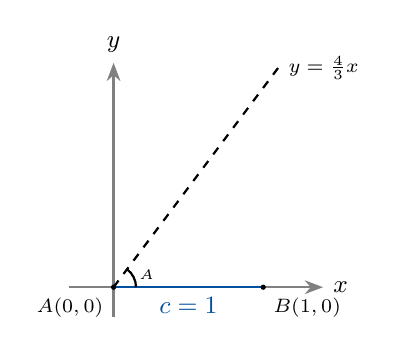
\begin{tikzpicture}[scale=1.9, >=Stealth, line width=0.8pt]
    \draw[->, gray] (-0.3, 0) -- (1.4, 0) node[right, text=black] {\small $x$};
    \draw[->, gray] (0, -0.2) -- (0, 1.5) node[above, text=black] {\small $y$};
    \coordinate (A) at (0,0);
    \coordinate (B) at (1,0);
    \draw[thick, mainblue] (A) -- (B) node[midway, below] {\small $c=1$};
    \fill (A) circle (0.5pt) node[below left, font=\scriptsize] {$A(0,0)$};
    \fill (B) circle (0.5pt) node[below right, font=\scriptsize] {$B(1,0)$};
    \coordinate (RayEnd) at (1.1, 1.466);
    \draw[dashed, thick] (A) -- (RayEnd);
    \node[right, font=\scriptsize] at (RayEnd) {$y=\frac{4}{3}x$};
    \draw (0.15,0) arc (0:53.13:0.15);
    \node[font=\tiny] at (0.22, 0.08) {$A$};
\end{tikzpicture}
\\ \vspace{-0.5em} \tiny 图 1：标准化与参数化后的初始几何模型
\end{minipage}

\subsection{约束一：保证 $\angle B < 90^\circ$（确定上限）}
\begin{minipage}[c]{0.56\textwidth}
为使 $\angle B$ 为锐角，点 $C$ 在 $x$ 轴上的投影必须严格位于点 $B$ 的左侧。即点 $C$ 必须位于过点 $B$ 的垂线 $x=1$ 的左侧（$x_C < 1$）。
\end{minipage}\hfill
\begin{minipage}[c]{0.41\textwidth}
\centering
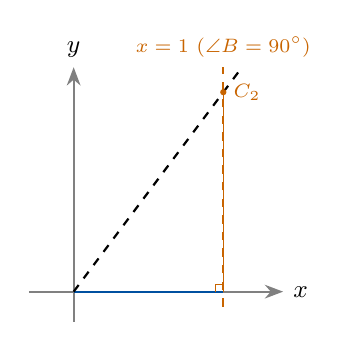
\begin{tikzpicture}[scale=1.9, >=Stealth, line width=0.8pt]
    \draw[->, gray] (-0.3, 0) -- (1.4, 0) node[right, text=black] {\small $x$};
    \draw[->, gray] (0, -0.2) -- (0, 1.5) node[above, text=black] {\small $y$};
    \coordinate (A) at (0,0);  \coordinate (B) at (1,0);
    \draw[thick, mainblue] (A) -- (B);
    \coordinate (RayEnd) at (1.1, 1.466); \draw[dashed, thick] (A) -- (RayEnd);
    
    % 边界
    \draw[mainorange, dashed, thick] (1,-0.1) -- (1, 1.5);
    \node[above, font=\scriptsize, mainorange] at (1, 1.5) {$x=1\ (\angle B = 90^\circ)$};
    \coordinate (C2) at (1, 1.333);
    \fill[mainorange] (C2) circle (0.6pt) node[right, font=\scriptsize] {$C_2$};
    \draw[mainorange, thin] (B) -- (C2);
    \draw[mainorange, thin] (0.95, 0) -- (0.95, 0.05) -- (1, 0.05);
\end{tikzpicture}
\\ \vspace{-0.5em} \tiny 图 2：当 $C$ 位于 $C_2$ 时达到上限，得 $b = AC_2 = \frac{5}{3}$
\end{minipage}

\subsection{约束二：保证 $\angle C < 90^\circ$（确定下限）}
\begin{minipage}[c]{0.56\textwidth}
根据直径圆周角定理，以 $AB$ 为直径作圆，该圆边界上的点对 $AB$ 的张角严格为 $90^\circ$。为使 $\angle C$ 为锐角，点 $C$ 必须严格位于该圆外部。
\end{minipage}\hfill
\begin{minipage}[c]{0.41\textwidth}
\centering
\begin{tikzpicture}[scale=1.9, >=Stealth, line width=0.8pt]
    \draw[->, gray] (-0.3, 0) -- (1.4, 0) node[right, text=black] {\small $x$};
    \draw[->, gray] (0, -0.2) -- (0, 1.1) node[above, text=black] {\small $y$};
    \coordinate (A) at (0,0);  \coordinate (B) at (1,0);
    \draw[thick, mainblue] (A) -- (B);
    \coordinate (RayEnd) at (0.8, 1.066); \draw[dashed, thick] (A) -- (RayEnd);
    
    % 边界
    \draw[mainred, dashed, thick] (1,0) arc (0:180:0.5);
    \node[mainred, font=\scriptsize] at (0.5, 0.6) {直径圆 ($\angle C = 90^\circ$)};
    \coordinate (C1) at (0.36, 0.48);
    \fill[mainred] (C1) circle (0.6pt) node[above left, font=\scriptsize] {$C_1$};
    \draw[mainred, thin] (B) -- (C1);
    \coordinate (C1_A_proj) at ($(C1)!0.08!(A)$);
    \coordinate (C1_B_proj) at ($(C1)!0.08!(B)$);
    \coordinate (C1_corner) at ($(C1_A_proj) + (C1_B_proj) - (C1)$);
    \draw[mainred, thin] (C1_A_proj) -- (C1_corner) -- (C1_B_proj);
\end{tikzpicture}
\\ \vspace{-0.5em} \tiny 图 3：当 $C$ 位于 $C_1$ 时达到下限，在 $\text{Rt}\triangle AC_1B$ 中，$b = AC_1 = \cos A = \frac{3}{5}$
\end{minipage}

\subsection{轨迹锁定与求解}
\begin{minipage}[c]{0.56\textwidth}
综合上述约束条件，点 $C$ 的合法活动范围被严格锁定在射线上的线段 $C_1C_2$ 之内（不含端点）。

由图可知 $b \in \left(\frac{3}{5}, \frac{5}{3}\right)$。从而目标式 $\frac{b}{2c} = \frac{b}{2} \in \left(\frac{3}{10}, \frac{5}{6}\right)$。
\end{minipage}\hfill
\begin{minipage}[c]{0.41\textwidth}
\centering
\begin{tikzpicture}[scale=1.9, >=Stealth, line width=0.8pt]
    \draw[->, gray] (-0.3, 0) -- (1.4, 0) node[right, text=black] {\small $x$};
    \draw[->, gray] (0, -0.2) -- (0, 1.5) node[above, text=black] {\small $y$};
    \coordinate (A) at (0,0); \coordinate (B) at (1,0);
    \draw[thick, mainblue] (A) -- (B);
    \coordinate (RayEnd) at (1.1, 1.466); \draw[dashed, thick, gray] (A) -- (RayEnd);
    
    \draw[mainred, dashed, thick] (1,0) arc (0:180:0.5);
    \draw[mainorange, dashed, thick] (1,-0.1) -- (1, 1.5);
    
    \coordinate (C1) at (0.36, 0.48);
    \coordinate (C2) at (1, 1.333);
    
    % 合法轨迹
    \draw[maingreen, line width=3.0pt, cap=round] (C1) -- (C2);
    \draw[<-, thick, black] (0.68, 0.906) -- ++(-0.25, 0.25) node[above, font=\tiny, align=center] {合法轨迹 $C_1C_2$\\$b \in \left(\frac{3}{5}, \frac{5}{3}\right)$};
    
    \fill[mainred] (C1) circle (0.6pt) node[below right, font=\scriptsize] {$C_1$};
    \fill[mainorange] (C2) circle (0.6pt) node[right, font=\scriptsize] {$C_2$};
\end{tikzpicture}
\\ \vspace{-0.5em} \tiny 图 4：可行域的几何呈现
\end{minipage}

\section{本题本质：数学建模全流程升华}
回顾上述解答，这并非简单的“画图找边界”技巧，而是一个极其经典的\textbf{数学建模与转化过程}。我们经历了以下五个严密的逻辑推演步骤：

\vspace{0.15cm}
\begin{center}
    \begin{tikzpicture}[node distance=0.85cm, auto, >={Stealth[scale=0.95]}]
        \tikzstyle{stepbox} = [draw=black!70, fill=gray!10, rectangle, thick, rounded corners=2pt, inner sep=4.5pt, text centered, font=\sffamily\small]
        
        \node[stepbox] (s1) {第一步：利用相似性消除尺度 $\Rightarrow$ \textbf{齐次化}};
        \node[stepbox, below=0.25cm of s1] (s2) {第二步：建立坐标系固定标准模型 $\Rightarrow$ \textbf{标准化}};
        \node[stepbox, below=0.25cm of s2] (s3) {第三步：用动点 $C$ 描述所有三角形 $\Rightarrow$ \textbf{参数化}};
        \node[stepbox, below=0.25cm of s3] (s4) {第四步：将锐角约束转化为图形边界 $\Rightarrow$ \textbf{约束转化}};
        \node[stepbox, below=0.25cm of s4] (s5) {第五步：在轨迹可行域上求距离极值 $\Rightarrow$ \textbf{几何最值}};
        
        \draw[->, thick] (s1) -- (s2);
        \draw[->, thick] (s2) -- (s3);
        \draw[->, thick] (s3) -- (s4);
        \draw[->, thick] (s4) -- (s5);
    \end{tikzpicture}
\end{center}
\vspace{0.15cm}

\begin{conceptbox}{结语}
透过这道题，应当深刻体会高级解题视角的威力所在：\\
\centerline{\textbf{“一道复杂的三角函数范围题，竟然可以完全不碰三角函数化简。”}}\\
从代数比值到几何轨迹，正是数学证明中化繁为简、形数结合的极致体现。
\end{conceptbox}

\newpage

\section{第二部分：经典模型拓展——固定对边与对角的范围与最值}

在上一部分中，我们通过固定单边 $c=1$ 与角度 $\angle A$，探讨了动点 $C$ 在射线上的线性轨迹。
本部分我们将该“轨迹思想”进一步推广至解三角形中最经典的\textbf{“定对边对角”（固定对边与对角）}模型，并对比三种通解方法。

\subsection{1. 核心模型与方法对比}
在锐角 $\triangle ABC$ 中，已知对边 $c = 2$，对角 $C = \dfrac{\pi}{3}$，其中 $a, b, c$ 分别是角 $A, B, C$ 的对边。试讨论以下三个对称式：
\[
a+b, \qquad ab, \qquad a^2+b^2
\]
的取值范围或最值。

对于“定对边对角”求最值/范围问题，我们通常有以下三种行之稳定的工具：
\begin{center}
\renewcommand{\arraystretch}{1.25}
\begin{tabularx}{\linewidth}{>{\bfseries}p{2.5cm} X X}
\toprule
方法名称 & 适用场景 & 方法特点与优缺点 \\
\midrule
轨迹法（几何直观） & 选择题、填空题，或快速突破几何直观 & \textbf{优点}：直观快速，可一眼看清对称最值与端点开闭。\\
 & & \textbf{缺点}：在解答题中直接作为证明步骤时，轨迹方程的推导与叙述较为繁琐。\\
\midrule
正弦定理 + \par 一角一函数 & 解答题通解，特别是求完整区间范围或非对称式（如 $2a+b$） & \textbf{优点}：代数推导极其严密，适用面最广，能精确确定开闭区间的端点值。\\
 & & \textbf{缺点}：三角恒等变形及辅助角公式的计算量较大，易错。\\
\midrule
余弦定理 + \par 基本不等式 & 快速求单侧最值（如求最大值） & \textbf{优点}：代数书写最为简练，不容易出错。\\
 & & \textbf{缺点}：只能求出单侧最值，在非对称或开区间求完整边界时力不从心。\\
\bottomrule
\end{tabularx}
\end{center}

\begin{conceptbox}{关于“锐角三角形”的边界限定（注意）}
题目中明确指出 $\triangle ABC$ 是\textbf{锐角三角形}。由于 $C = \dfrac{\pi}{3}$ 已经是锐角，所以临界状态是 $\angle A \to 90^\circ$ 或 $\angle B \to 90^\circ$。在直角三角形的临界点上，边界值是\textbf{取不到的}（开区间）。因此，求范围时下端必须是开区间，不能写成最小值。
\end{conceptbox}

\subsection{2. 轨迹法：定弦定角对应的圆弧轨迹}
根据圆周角定理，当三角形的底边 $AB$（弦）固定，且对角 $\angle ACB$ 恒定时，顶点 $C$ 的运动轨迹是一段\textbf{以 $AB$ 为弦的圆弧}。

\begin{minipage}[c]{0.52\textwidth}
由于 $c=2, C = \dfrac{\pi}{3}$。由正弦定理，外接圆直径为：
\[
2R = \frac{c}{\sin C} = \frac{2}{\sin\frac{\pi}{3}} = \frac{4}{\sqrt{3}} \implies R = \frac{2}{\sqrt{3}}
\]
我们在平面直角坐标系中，令底边 $AB$ 落在 $x$ 轴上，且 $A(-1,0), B(1,0)$（以保证 $AB = c = 2$）。
此时，外接圆的圆心为 $O_c\left(0, \dfrac{1}{\sqrt{3}}\right)$，半径 $R = \dfrac{2}{\sqrt{3}}$。
圆的方程为：
\[
x^2 + \left(y - \frac{1}{\sqrt{3}}\right)^2 = \frac{4}{3}
\]
当 $\triangle ABC$ 为锐角三角形时：
\begin{enumerate}
  \item 为保证 $\angle A < 90^\circ$，点 $C$ 必须在过点 $A$ 的垂线 $x = -1$ 右侧。
  \item 为保证 $\angle B < 90^\circ$，点 $C$ 必须在过点 $B$ 的垂线 $x = 1$ 左侧。
\end{enumerate}
故点 $C$ 的合法轨迹被锁定在 $x \in (-1, 1)$ 的圆弧上。
\end{minipage}\hfill
\begin{minipage}[c]{0.45\textwidth}
\centering
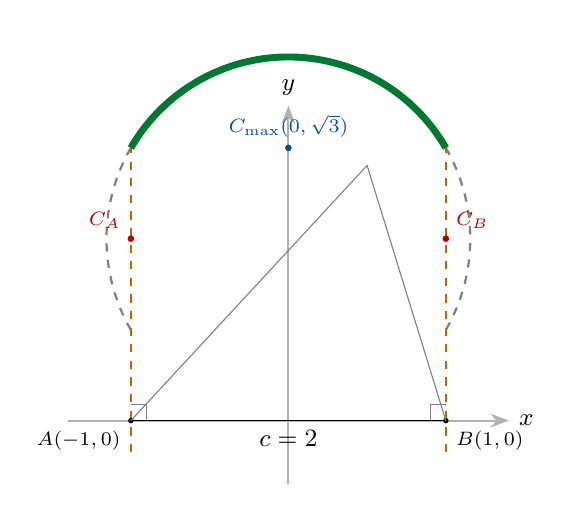
\begin{tikzpicture}[scale=2.0, >=Stealth, line width=0.8pt]
    % 坐标轴
    \draw[->, gray!60] (-1.4, 0) -- (1.4, 0) node[right, text=black] {\small $x$};
    \draw[->, gray!60] (0, -0.4) -- (0, 2.0) node[above, text=black] {\small $y$};
    
    \coordinate (A) at (-1,0);
    \coordinate (B) at (1,0);
    \coordinate (Oc) at (0, 0.577);
    
    % 画圆弧 (定对角 C = 60度 对应的整个弧，从 B(-30度) 到 A(210度))
    \draw[dashed, gray] ([shift=(Oc)] -30:1.155) arc (-30:30:1.155);
    \draw[dashed, gray] ([shift=(Oc)] 150:1.155) arc (150:210:1.155);
    
    % 边界垂线
    \draw[dashed, mainorange] (-1, -0.2) -- (-1, 1.8);
    \draw[dashed, mainorange] (1, -0.2) -- (1, 1.8);
    
    % 边界直角标记
    \draw[thin, gray] (-1, 0.1) -- (-0.9, 0.1) -- (-0.9, 0);
    \draw[thin, gray] (1, 0.1) -- (0.9, 0.1) -- (0.9, 0);
    
    % 边界交点
    \coordinate (CA) at (-1, 1.155);
    \coordinate (CB) at (1, 1.155);
    \coordinate (Cmax) at (0, 1.732);
    
    % 合法圆弧轨迹 (30度到150度)
    \draw[maingreen, line width=2.5pt] ([shift=(Oc)] 30:1.155) arc (30:150:1.155);
    
    % 顶点
    \fill (A) circle (0.5pt) node[below left, font=\scriptsize] {$A(-1,0)$};
    \fill (B) circle (0.5pt) node[below right, font=\scriptsize] {$B(1,0)$};
    \fill[mainred] (CA) circle (0.6pt) node[above left, font=\scriptsize] {$C_A$};
    \fill[mainred] (CB) circle (0.6pt) node[above right, font=\scriptsize] {$C_B$};
    \fill[mainblue] (Cmax) circle (0.6pt) node[above, font=\scriptsize] {$C_{\max}(0, \sqrt{3})$};
    
    \draw[thin] (A) -- (B) node[midway, below] {\small $c=2$};
    
    % 示意三角形
    \draw[thin, gray] (A) -- (0.5, 1.62) -- (B);
    
\end{tikzpicture}
\\ \vspace{-0.5em} \tiny 图 5：定弦定角下的点 $C$ 圆弧轨迹与锐角边界
\end{minipage}

\vspace{0.2cm}
\textbf{轨迹法分析最值：}\\
当点 $C$ 处于对称中心，即 $C$ 位于圆弧的中点 $C_{\max}(0, \sqrt{3})$ 时，$\triangle ABC$ 为等边三角形（$a = b = c = 2$），此时三角形的周长、面积及各项对称代数式均达到最大值：
\begin{itemize}
  \item $(a+b)_{\max} = 2+2 = 4$
  \item $(ab)_{\max} = 2 \times 2 = 4$
  \item $(a^2+b^2)_{\max} = 2^2+2^2 = 8$
\end{itemize}

当点 $C$ 趋近于左右两个临界边界点 $C_A$ 或 $C_B$（即直角三角形状态，此时 $a,b$ 分别趋近于 $\frac{2}{\sqrt{3}}$ 和 $\frac{4}{\sqrt{3}}$）时，各项代数式无限趋近于下确界（开区间端点）：
\begin{itemize}
  \item $a+b > \frac{2}{\sqrt{3}} + \frac{4}{\sqrt{3}} = 2\sqrt{3}$
  \item $ab > \frac{2}{\sqrt{3}} \times \frac{4}{\sqrt{3}} = \frac{8}{3}$
  \item $a^2+b^2 > \left(\frac{2}{\sqrt{3}}\right)^2 + \left(\frac{4}{\sqrt{3}}\right)^2 = \frac{20}{3}$
\end{itemize}

从而，我们直观地锁定三者的取值区间分别为：
\[
a+b \in (2\sqrt{3}, 4], \qquad ab \in \left(\frac{8}{3}, 4\right], \qquad a^2+b^2 \in \left(\frac{20}{3}, 8\right]
\]

\begin{conceptbox}{为什么轨迹法仅适用于“对称式”？}
轨迹法之所以在此处如此敏捷，是因为 $a+b, ab, a^2+b^2$ 均为关于 $a,b$ 的\textbf{对称代数式}。
在几何上，当点 $C$ 在对称轴上时，对称式的最值能够同步取得。
如果题目要求 $2a+b$ 的范围，由于 $2a+b \ne 2b+a$（非对称），其最大值点绝对不在等边三角形处取得，此时轨迹法便无法直接判定最值位置。我们必须使用下面的正弦定理代数通解法。
\end{conceptbox}

\subsection{3. 正弦定理 + 一角一函数：大题最通用的代数通解}
通过正弦定理将边 $a, b$ 参数化为关于角 $A$ 的三角函数：

由正弦定理：
\[
\frac{a}{\sin A} = \frac{b}{\sin B} = \frac{c}{\sin C} = \frac{2}{\sin\frac{\pi}{3}} = \frac{4}{\sqrt{3}}
\]
可得边的参数化表示：
\[
a = \frac{4}{\sqrt{3}}\sin A, \qquad b = \frac{4}{\sqrt{3}}\sin B
\]
由于 $A + B + C = \pi$ 且 $C = \frac{\pi}{3}$，所以 $B = \frac{2\pi}{3} - A$。
从而有：
\[
b = \frac{4}{\sqrt{3}}\sin\left(\frac{2\pi}{3} - A\right)
\]

\textbf{第一步：锁定角 $A$ 的取值范围}\\
因为 $\triangle ABC$ 为锐角三角形，必须满足：
\[
\begin{cases}
  0 < A < \frac{\pi}{2} \\
  0 < B < \frac{\pi}{2} \implies 0 < \frac{2\pi}{3} - A < \frac{\pi}{2}
\end{cases}
\implies
\begin{cases}
  0 < A < \frac{\pi}{2} \\
  \frac{\pi}{6} < A < \frac{2\pi}{3}
\end{cases}
\implies A \in \left(\frac{\pi}{6}, \frac{\pi}{2}\right)
\]
这即是后续求值域的自变量核心范围。

\textbf{第二步：求解各式的取值范围}
\begin{enumerate}
  \item \textbf{求解 $a+b$ 的范围}：
    \[
    a+b = \frac{4}{\sqrt{3}}\left[ \sin A + \sin\left(\frac{2\pi}{3} - A\right) \right]
    \]
    利用和差化积或两角和公式展开：
    \[
    \sin A + \sin\left(\frac{2\pi}{3} - A\right) = 2\sin\frac{\pi}{3}\cos\left(A - \frac{\pi}{3}\right) = \sqrt{3}\cos\left(A - \frac{\pi}{3}\right)
    \]
    从而有：
    \[
    a+b = 4\cos\left(A - \frac{\pi}{3}\right)
    \]
    由于 $A \in \left(\frac{\pi}{6}, \frac{\pi}{2}\right)$，所以 $A - \frac{\pi}{3} \in \left(-\frac{\pi}{6}, \frac{\pi}{6}\right)$。
    此时 $\cos\left(A - \frac{\pi}{3}\right) \in \left(\frac{\sqrt{3}}{2}, 1\right]$。
    故：
    \[
    a+b \in \left(2\sqrt{3}, 4\right]
    \]

  \item \textbf{求解 $ab$ 的范围}：
    \[
    ab = \frac{16}{3}\sin A\sin\left(\frac{2\pi}{3} - A\right) = \frac{16}{3}\sin A\left(\frac{\sqrt{3}}{2}\cos A + \frac{1}{2}\sin A\right) = \frac{8}{3}\sin^2 A + \frac{8}{\sqrt{3}}\sin A\cos A
    \]
    利用降幂公式与倍角公式：
    \[
    ab = \frac{4}{3}(1 - \cos 2A) + \frac{4}{\sqrt{3}}\sin 2A = \frac{4}{3} + \frac{8}{3}\left(\frac{\sqrt{3}}{2}\sin 2A - \frac{1}{2}\cos 2A\right)
    \]
    \[
    ab = \frac{4}{3} + \frac{8}{3}\sin\left(2A - \frac{\pi}{6}\right)
    \]
    由于 $A \in \left(\frac{\pi}{6}, \frac{\pi}{2}\right)$，so $2A - \frac{\pi}{6} \in \left(\frac{\pi}{6}, \frac{5\pi}{6}\right)$。
    此时 $\sin\left(2A - \frac{\pi}{6}\right) \in \left(\frac{1}{2}, 1\right]$。
    故：
    \[
    ab \in \left(\frac{4}{3} + \frac{8}{3} \times \frac{1}{2}, \ \frac{4}{3} + \frac{8}{3} \times 1\right] \implies ab \in \left(\frac{8}{3}, 4\right]
    \]

  \item \textbf{求解 $a^2+b^2$ 的范围}：
    直接利用前面得到的 $ab$ 范围以及余弦定理关系式 $a^2+b^2 - ab = 4 \implies a^2+b^2 = 4 + ab$。
    由于 $ab \in \left(\frac{8}{3}, 4\right]$，直接可得：
    \[
    a^2+b^2 \in \left(\frac{20}{3}, 8\right]
    \]
\end{enumerate}

\subsection{4. 余弦定理 + 基本不等式：解答题中求最值的捷径}
如果题目不要求求解完整的区间范围，而仅询问最大值，那么余弦定理结合基本不等式是最为简洁的方法。

由余弦定理：
\[
c^2 = a^2+b^2 - 2ab\cos C \implies 4 = a^2+b^2 - ab
\]

\begin{enumerate}
  \item \textbf{求 $a+b$ 的最大值}：
    因为 $4 = (a+b)^2 - 3ab$。
    由基本不等式 $ab \le \left(\dfrac{a+b}{2}\right)^2$，有：
    \[
    4 \ge (a+b)^2 - 3 \times \frac{(a+b)^2}{4} = \frac{(a+b)^2}{4} \implies (a+b)^2 \le 16 \implies a+b \le 4
    \]
    当且仅当 $a = b = 2$ 时等号成立，故最大值为 4。

  \item \textbf{求 $ab$ 的最大值}：
    因为 $4 = a^2+b^2 - ab$。
    由基本不等式 $a^2+b^2 \ge 2ab$，有：
    \[
    4 \ge 2ab - ab = ab \implies ab \le 4
    \]
    当且仅当 $a = b = 2$ 时等号成立，故最大值为 4。

  \item \textbf{求 $a^2+b^2$ 的最大值}：
    因为 $ab \le \frac{a^2+b^2}{2}$。
    代入余弦式：
    \[
    4 = a^2+b^2 - ab \ge a^2+b^2 - \frac{a^2+b^2}{2} = \frac{a^2+b^2}{2} \implies a^2+b^2 \le 8
    \]
    当且仅当 $a = b = 2$ 时等号成立，故最大值为 8。
\end{enumerate}

\begin{conceptbox}{方法局限性探讨}
基本不等式法在求最值时非常快捷，但它\textbf{无法给出一侧的开区间边界（即下确界）}。
例如，如果我们想通过基本不等式求 $ab$ 的下限，由于 $ab > 0$，我们顶多能得出 $ab > 0$，而无法得出在锐角约束下的精确下界 $\frac{8}{3}$。因此，求完整范围时仍应以正弦定理为首选。
\end{conceptbox}

\end{document}
